% Template for articles submitted to the International Journal of Forecasting
% Further instructions are available at www.ctan.org/pkg/elsarticle
% You only need to submit the pdf file, not the source files.
% If your article is accepted for publication, you will be asked for the source files.


\documentclass[11pt,3p,review,authoryear]{elsarticle}

\usepackage{listings}
\usepackage{color}
\usepackage{graphicx}
\usepackage{multirow}
\usepackage{array,rotating}
\usepackage{adjustbox}
\usepackage{numprint}
\usepackage{siunitx}
\usepackage{amsmath}


\definecolor{dkgreen}{rgb}{0,0.6,0}
\definecolor{gray}{rgb}{0.5,0.5,0.5}
\definecolor{dkred}{rgb}{0.6,0,0}

\lstset{frame=tb,
  language=R,
  aboveskip=3mm,
  belowskip=3mm,
  showstringspaces=false,
  columns=flexible,
  basicstyle={\small\ttfamily},
  numbers=none,
  numberstyle=\tiny\color{gray},
  keywordstyle=\color{blue},
  commentstyle=\color{dkgreen},
  stringstyle=\color{dkred},
  breaklines=true,
  breakatwhitespace=true,
  tabsize=3
}

\journal{International Journal of Forecasting}
\bibliographystyle{model5-names}
\biboptions{longnamesfirst}
% Please use \citet and \citep for citations.


\begin{document}

\begin{frontmatter}

\title{Fast and Accurate Yearly Time Series Forecasting with Forecast Combinations}

%% AUTHORS %%%%%%%%%%%%%%%%%%%%%%%%%%%%%%%%%%%%%%%%%%%%%%%%%%%%%%%%%%%%%%%%%%%%
%% Leave this section commented out so that the paper is blinded for review.
%% Group authors per affiliation:
% \author[ss]{David Shaub\corref{cor}}
% \address[ss]{Harvard University Extension School}


%% Only give the email address of the corresponding author
% \cortext[cor]{Corresponding author}
% \ead{davidshaub@g.harvard.edu}
%%%%%%%%%%%%%%%%%%%%%%%%%%%%%%%%%%%%%%%%%%%%%%%%%%%%%%%%%%%%%%%%%%%%%%%%%%%%%%%%


\begin{abstract}
Combination forecasting strategies have long been known to produce superior out-of-sample forecasting performance. In the M4 forecasting competition, a very simple forecast combination strategy achieved third place on yearly time series. An analysis of the ensemble model versus the component models suggests the competitive accuracy comes from avoiding poor forecasts instead of beating the best individual models. Moreover, the simple ensemble model fits very quickly, can easily scale horizontally with additional CPU cores or a cluster of computers, and can very quickly and easily be implemented by users. This approach might be of particular interest to users who need accurate yearly forecasts without significant time, resources, or expertise to tune models. Users of the R statistical programming language can access this modeling approach in the "forecastHybrid" package.
\end{abstract}

\begin{keyword}
Automatic forecasting\sep Combining forecasts\sep Evaluating forecasts\sep Forecasting competitions\sep Software
% Suggested keywords are listed at https://ijf.forecasters.org/keywords/
\end{keyword}

\end{frontmatter}


\section{Introduction}
Model selection presents a challenge for forecasters since selecting the incorrect model leads to additional forecasting error. One hedge against incorrect model specification is a forecast combination from several candidate models. Granger \& Bates \cite{BatesGranger1969} suggested such an approach and observed that somewhat surprisingly the combined forecast can even outperform the single best performing component forecast. While combination weights selected equally or proportionally to past model error are possible approaches, no shortage of more sophisticated combination schemes have been suggested. For example, instead of normalizing weights to sum to unity, unconstrained--and even negative--weights could be possible \citep{GrangerRamanathan1984}.


It might appear that the simplest approach of assigning equal weights to all component models is woefully obsolete and likely noncompetitive compared to the multitude of sophisticated combination approaches or advanced machine learning and neural network forecasting models. However, results from the 2018 M4 competition \citep{M4} show that such a simple approach can still be competitive, particularly for yearly time series where the method achieved third place. This paper, therefore, seeks to examine why such a simple combination procedure remains effective and proved competetive in the M4 competetion against more sophisticated models. Specifically it seeks to contribute to the understanding of how simple model combination performs relative to in-sample and oracle model selection procedures.


This article is organized as follows: section 2 describes the combination methodology, section 3 contains analysis of the performance characteristics of this model in the M4 competition versus individual models, and section 4 concludes.


\section{Methodology}
The author's submission for the M4 competetion utilized this combination strategy for only the yearly time series while for other frequencies (i.e. hourly, daily, weekly, monthly, quarterly) a temporal hierarchical approach using the "thief" R package \citep{ATHANASOPOULOS201760} was used. The analysis in this paper will, therefore, limit its scope to the perfomance of the combination strategy on the yearly time series in the M4 competetion.


The combination strategy employed in the M4 competition submission utilized the statistical programming language R \citep{Rlang} and leveraged the "forecastHybrid" \citep{forecastHybrid} package. The component models allowed in the "forecastHybrid" package are the  \lstinline{auto.arima} (automatic selection of AR, MA and integration order for seasonal time series), \lstinline{ets} (exponential smoothing with automatic additive/additive damped/multiplicative/multiplicative damped trend and seasonal components), \lstinline{thetaf} (the Theta model described in \citep{THETA}), \lstinline{nnetar} (a feedforward neural network with lags as features) \lstinline{stlm}(a simple seasonal and trend decomposion), \lstinline{tbats} (a state space model with Box-Cox transforms to handle scale invariance, Fourier transforms to handle complex and time-varying seasonality, and ARMA for error correction described in \citep{TBATS}), and \lstinline{snaive} (a seaonal naive forecast). All these models are provided by the "forecast" package \citep{Forecast}. The "forecastHybrid" package includes these component models to enhance the "forecast" package base models and allow easy ensembling.

The "forecastHybrid" package produces forecasts out to a horizon $h$ by applying a weight $w_m$ to each $m$ of the $n$ model forecasts in the ensemble. The ensemble forecast $f(i)$ for time horizon $1 \leq i \leq h$ and with individual component model forecasts $f_m(i)$ is then
\begin{align}
f(i) & = \sum_{m=1}^n w_m\cdot f_m(i)
\end{align}
The weights can be determined in several ways (i.e. supplied by the user, set equally, determined by in-sample errors, or determined by cross validation). For the M4 submission, the weights were set equally and automatically to $w_m = \frac{1}{n} = \frac{1}{3}$ since this method is the quickest. Perhaps surprisingly this simple average was enough to be competetive.

For the author's submission in the M4 competetion, only the \texttt(auto.arima), \texttt(thetaf), and \texttt(tbats) component models were included in the yearly ensemble. These models were selected from the author's experience as these models tend to produce reasonable forecasts; furtheremore, these models both can capture and have reasonable selection procedures that prevent the drastic overfitting that can occur on models with too many free coefficients. Furthermore, since a large number of time series needed to be forecasted with prediction intervals for the M4 competetion, performance was a concern. The \texttt{nnetar} model in particular could not be included--despite its favorable capability of handling nonlinear properties in the time series--since its empricial simulations for the prediction intervals are quite slow. The \texttt{ets} model was not included since \texttt{tbats} and \texttt{auto.arima} models should be able to capture any data generating process that the state space model hands well. Finally, the \texttt{stlm} seasonal decomposion was also deemed unnecessary since the author expected many structural breaks in the M4 time series that would not be handled well, and the \texttt{snaive} model was also deemed too simple to be competetive compared to machine learning techniques that could be used to learn across the 100,000 time series.

The following R code produces this forecast combination for a single yearly time series \lstinline{x} with a forecasting horizon \lstinline{h = 6} along with 95\% prediction intervals.
\begin{lstlisting}[language=R]
forecastM4 <- function(x, h = 6){
    return(forecast(hybridModel(x, models = "aft", verbose = FALSE),
                      h = h, level = 95, PI.combination = "mean"))
}
\end{lstlisting}

It should be noted, however, that the prediction intervals produced by this methodology are highly dubious: the prediction intervals from each individual component models are similarly averaged together with no account for any possible covariance, and in the M4 competition the approach overestimated the prediction intervals coverage. Since the M4 competition rules and prizes incentivized submission of prediction intervals, they were produced nonetheless, but the submission entry focused attention on the point forecasts.


The forecasting procedure can be parallelized to decrease the time to fit models. A user can apply this parallelization both within models and across time series. If a single time series needs to be fit, the three individual component model can each be fit in parallel on a separate CPU core/thread by passing the \texttt{parallel = TRUE} argument to the \texttt{hybridModel()} function; the \texttt{auto.arima} and \texttt{tbats} models can themselves also use parallel processing \footnote{For a more detailed description of the "forecastHybrid" package and its usage, refer to the package vignette at https://cran.r-project.org/web/packages/forecastHybrid/vignettes/forecastHybrid.html or the package reference manual at https://cran.r-project.org/web/packages/forecastHybrid/forecastHybrid.pdf}. Furthermore, when users need to fit a model and forecast many time series (such as the case of M4's 23000 yearly time series), this forecasting function can be run as a distributed map operation on multiple CPUs or machines in a cluster. For example, if we wish to utilize 16 threads on a server to forecast the M4 time series in a list \texttt{M4Yearly}, we could use the "pbapply" package \citep{pbapply} to map the forecasting task and also view a real-time progress bar with an estimated completion time\footnote{The following R code will use 12 processes/threads to forecast a list \texttt{M4Yearly} of yearly time series in parallel: \texttt{forecasts <- pblapply(M4Yearly, forecastM4, cl = 12)}}. The train and forecasting processing is fast: on an i7-8850H CPU with 6 cores and 12 threads the entire train and forecast procedure completes in approximately 55 minutes for the 23,000 yearly M4 time series which is about 7 time series per second.


In the M4 submission, this parallelization strategy was used, and the entire setup of the R environment, installation of dependencies packages, and download of the M4 dataset was packaged into a Docker container for reproducibility. The simplicity of this approach offers great flexibility to practitioners who need to adjust the latency of model training and forecasting without writing much custom or complex code. Indeed the author's M4 submission for all time series amounted to fewer than 100 lines of R code and did not employ prepossessing or filtering that can making deploying automated forecasting systems at scale in a production environment difficult and vulnerable to new and degenerate datasets with characteristics such as missing data, extreme values, zero variance, etc. Modeling approaches that require building features or training on an entire corpus of training data may not be so readily online or amenable to an "embarrassingly parallel" workflow or easily-tunable user selection whether to apply parallelization within models or across time series.


\section{Analysis}
We might reasonably question why such a simple and well-known technique of averaging forecasts proved competitive in the M4 yearly time series. One hypothesis is that model selection is a difficult problem and more complex forecasting methodologies struggle to select a model that will perform well on out-of-sample data. The model selection problem for complex models could manifest itself as either the explicit selection in a candidate pool of models (or the weights assigned to these models if using more than one) or the implicit problem of selecting the optimal hyperparameters if a single, complex model is used that has many possible tuning parameters such as neural networks. The examination that follows supports this hypothesis and shows that the mean ensemble approach achieves competitive performance not by producing forecasts that barely miss the actual values but rather by producing fewer forecasts that very badly miss the actual values.


Three separate modeling strategies will be examined here. The first is the ensemble approach that was used in the M4 submission and that was described in section 2. The second is a model selection procedure that attempts to choose a single best model for the forecasting period based on the individual model that performs best on a holdout set created in the M4 train data. Since the M4 forecasting horizon is 6 for the yearly data, the final six observations of a time series are removed and each individual component model (\texttt{auto.arima}, \texttt{thetam}, and \texttt{tbats}) estimated on the truncated train time series. Each model then forecasts against the six observations, and the best individual model based on mean absolute scaled error (MASE) is selected and retrained on the full, original train time series. If multiple models have equivalent minimum MASE (as happens for constant, linear trend, or other time series that each model can perfectly predict on the holdout set), a single component model is randomly selected from those with the best MASE. The third and final model for comparison is a reference oracle model that is the individual component model for each time series that performs best on the M4 competition evaluation set. This final model is built not as a legitimate contender for a modeling strategy that could be used in practice for forecasting but rather to evaluate the efficacy of the second model selection procedure and as a benchmark to compare the accuracy of our forecasts against the best we might hope to do in some sense--at least with a single component model from the set of candidate models we examine here.

% latex table generated in R 3.5.1 by xtable 1.8-3 package
% Sat Oct  6 20:29:03 2018
\begin{table}[ht]
\centering
\begin{adjustbox}{width=1\textwidth}
\begin{tabular}{rrrrrrrrrrrr}
  \hline
 & Sensitivity/Recall & Specificity & Pos Pred Value & Neg Pred Value & Precision & Prevalence &  Balanced Accuracy \\ 
  \hline
Class: Arima & 0.20 & 0.78 & 0.29 & 0.69 & 0.29 & 0.31 & 0.49 \\ 
  Class: BATS & 0.16 & 0.83 & 0.31 & 0.68 & 0.31 & 0.32 & 0.50 \\ 
  Class: Theta & 0.61 & 0.37 & 0.36 & 0.61 & 0.36 & 0.37 & 0.49 \\ 
   \hline
\end{tabular}
\end{adjustbox}
\caption{Performance metrics for the model selection procedures}\label{tab:a}
\end{table}

% Distribution of log(MASE) for ensemble and selected models
\begin{figure}[h]
\centering
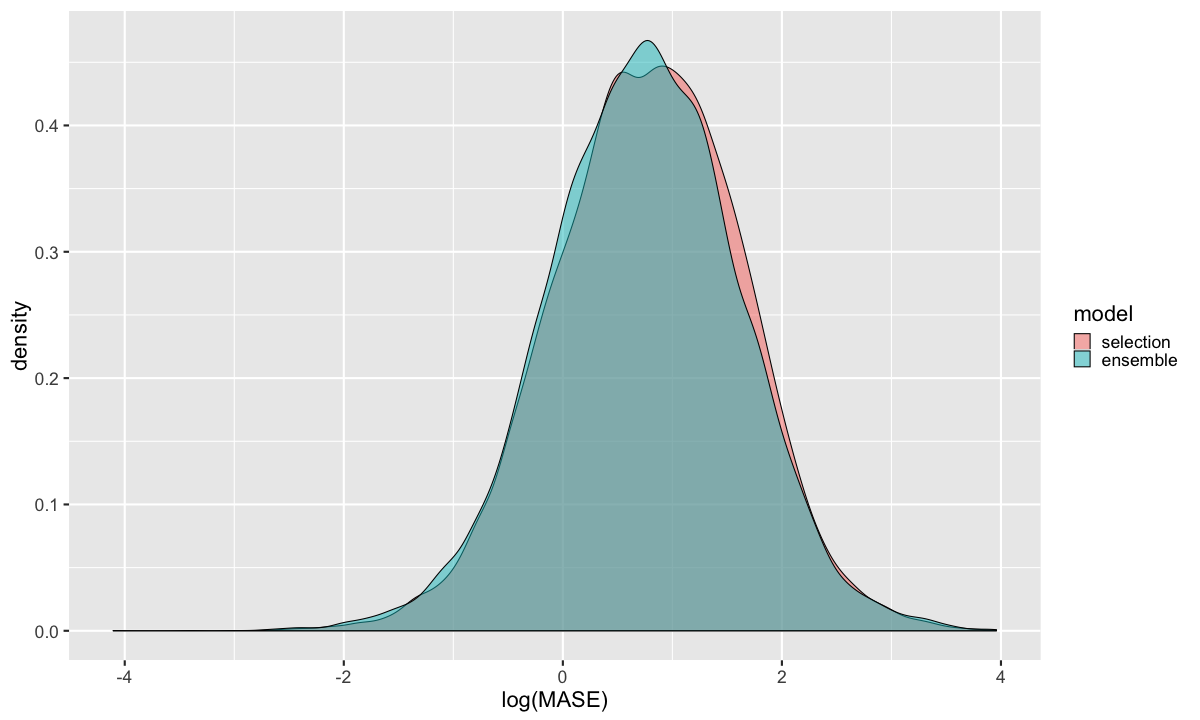
\includegraphics[width=\textwidth]{distribution}
\caption{Distribution of MASE for the ensemble and model selection forecasting procedures}\label{fig:a}
\end{figure}

% Table distribution of MASE for ensemble, oracle, and selection
\begin{table}[ht]
\centering
\npdecimalsign{.}
\nprounddigits{3}
\begin{tabular}{rrrrrrr}
\hline
& Min & 1st Quartile & Median & Mean & 3rd Quartile & Max\\
\hline
Reference \vline & 0.000 & 0.852 & 1.503 & 2.275 & 2.669 & 51.521\\
Selection \vline & 0.000 & 1.235 & 2.224 & 3.133 & 3.953 & 51.521 \\
Ensemble \vline & 0.0505 & 1.170 & 2.104 & 3.039 & 3.722 & 52.414\\
\hline
\end{tabular}
\caption{MASE summary statistics for the oracle reference, selection, and ensemble models}\label{tab:c}
\end{table}

% Table of Oracle model selection and best individual model
% latex table generated in R 3.5.1 by xtable 1.8-3 package
% Sat Oct  6 19:24:20 2018
\begin{table}[ht]
\centering
\begin{tabular}{rrrr}
  \hline
  & \multicolumn{3}{c}{\textbf{Reference}} \\
 \textbf{Selected} & Arima & BATS & Theta  \\
 \hline
 Arima & 1397 & 1486 & 1935 \\ 
   BATS & 1213 & 1197 & 1450 \\ 
  Theta & 4491 & 4613 & 5218 \\ 
   \hline
\end{tabular}
\caption{Reference best individual model on test set versus model from selection procedure}\label{tab:b}
\end{table}

Table~\ref{tab:c} and Figure~\ref{fig:a} shows the distribution of MASE for the models. In particular we can see that the ensemble model produces fewer forecasts with larger MASE compared with the selection procedure; the benefit appears to be most noteworthy around the third quartile. Both these approaches fall far short of the oracle reference model, however, indicating that if a model selection procedure could achieve high sensitivity and accuracy in selecting the correct model, we could expect substantial improvements in forecasting accuracy over the ensemble method. 


The model selection procedure employed here performs poorly and in fact worse than a naive approach of using the dominant class Theta model for every time series without bothering to evaluate performance on a holdout set. To be fair, a forecaster would not know \textit{a priori} when constructing forecasts that the Theta model would be the best individual model on the M4 yearly series. On the other hand, the Theta model was the best model in the M3 competition and even served as a benchmark model according to the M4 competition rules, so the empirical result that it is the majority class here is very surprising.

The Theta model is the best individual model for 37.4 percent of the time series while the selection procedure yields only 33.97 percent accuracy. The 95 percent confidence intervals for the selection procedure's accuracy encompasses 33.35 percent to 34.58 percent. Table~\ref{tab:a} highlights performance metrics of the model selection procedure. Indeed the balanced class accuracies hover below 50 percent and other metrics such as sensitivity and specificity show no evidence that the approach can select the correct model or avoid selecting an incorrect model. The sensitivity/recall and the precision metrics show predictions of the Theta model from the selection procedure are more likely to be correct than predictions for the other models; this is not surprising given the Theta model is the dominant class, but the specificity metric shows that the selection procedure achieves its sensitivity and precision metric performance by selecting the Theta model for far more time series than it should.

A confusion matrix is useful to view the distribution of the selected model versus the actual correct reference model that an oracle with access to the test set would select. If the selected model frequently corresponded to the correct reference model, we would expect large counts on the matrix diagonal. A visual inspection of the confusion matrix in Table~\ref{tab:b} confirms our analysis earlier, and we see that the selection procedure highly favors the Theta model. The lack of correlation in confusion matrix demonstrates the selection procedure's failure to identify the best model for the test period and that a dominant form of failure is the aggressive selection of the Theta model. McNemar's test \citep{MCNEMAR} for any improvement over the "no information rate" confirms this: the test produces a P-value less than \num{2e-16} giving us no reason to believe the selection procedure produces any improvement over the naive, majority-class approach. In summary, these results are consistent with research that shows that model selection strategies using only the current time series to be forecasted are fraught with risk of failure. Alternative approaches that examine the characteristics from multiple time series such as building time series features in \cite{modelSelection} might yield better results.



\section{Conclusion}
It might sound trivial to state that the way to produce good forecasts is to avoid making bad forecasts, but choosing a single model that will perform well on the test set based on the models' performance on the train set yields no improvement over the no information rate in the M4 yearly time series data. An examination of a simple ensemble forecasting method shows that equal arithmetic averaging of base models can serve of a hedge of model selection risk and help prevent some large forecasting errors.


This simple combination approach can be of particular interest to business users and software engineers who need to forecast a large number of time series automatically, without intervention, and without a global model that needs retraining with the addition of new time series or data drawn from a new data generating process. Finally, unlike many other approaches--and most machine learning approaches in particular--users with access to a large number of CPU cores or threads will find this simple combination approach from the "forecastHybrid" package attractive since both the training and forecasting scale linearly with the number of processes to reduce the duration required to forecast the collection of time series.

Finally, we might wonder about possible improvements to the combination weights used in the M4 submission and described in this article. Indeed the "forecastHybrid" package can use alternative combination weight strategies of user-supplied weights, in-sample error weights, or cross validated weights. The possibility of user-supplied weights would allow some exogenous weight selection algorithm to run and then conveniently produce forecasts by supplying these to the \texttt{hybridModel} function. There is reason to believe that weights selected by cross validation would perform better than this simple averaging approach since it would avoid overfitting problems typically experienced with weight selection on the train set and the underfitting that comes from giving performant models too little weight in the ensemble. We could also imagine a scenario where separate model weights apply to each forecast horizon (e.g. an ARIMA model receives more weight to capture short-term forecasting dynamics, but for a longer horizons a simple stasonal decomposiion model receives more weight due to its avoidance of explosive-growth forecasts that might come from the ARIMA model).

The source code and scripts used to produce all forecasts and analysis is available on the author's GitHub at (REDACTED URL FOR ANONYMOUS REVIEW).

\section*{Acknowledgments}

This research did not receive any specific grant from funding agencies in the public, commercial, or not-for-profit sectors.


% Bibliography.
\section{References}
\bibliography{ForecastHybrid}
\end{document}
